% !TEX TS-program = pdflatexmk
\documentclass[12pt]{article}

% Layout.
\usepackage[top=.75in, bottom=0.75in, left=.75in, right=.75in, headheight=1in, headsep=6pt]{geometry}

% Fonts.
\usepackage{mathptmx}
\usepackage[scaled=0.86]{helvet}
\renewcommand{\emph}[1]{\textsf{\textbf{#1}}}

% Misc packages.
\usepackage{amsmath,amssymb,latexsym}
\usepackage{graphicx}
\usepackage{array}
\usepackage{xcolor}
\usepackage{multicol}
\usepackage{tabularx,colortbl}
\usepackage{enumitem}
%to make tikz pics work
\usepackage{tikz,pgfplots}

\usepackage[colorlinks=true]{hyperref}

% Paragraph spacing
\parindent 0pt
\parskip 6pt plus 1pt
\def\tableindent{\hskip 0.5 in}
\def\ts{\hskip 1.5 em}

\usepackage{fancyhdr}
\pagestyle{fancy} 
\lhead{\large\sf\textbf{MATH F251 }}
\rhead{\large\sf\textbf{Calculus I}}
\chead{\large\sf\textbf{Homework 1}}

\newcommand{\localhead}[1]{\par\smallskip\textbf{#1}\nobreak\\}%
\def\heading#1{\localhead{\large\emph{#1}}}
\def\subheading#1{\localhead{\emph{#1}}}

\newenvironment{clist}%
{\bgroup\parskip 0pt\begin{list}{$\bullet$}{\partopsep 4pt\topsep 0pt\itemsep -2pt}}%
{\end{list}\egroup}%

\usetikzlibrary{calc}
\pgfplotsset{my style/.append style={axis x line=middle, axis y line=
middle, xlabel={$x$}, ylabel={$y$}, axis equal }}

\begin{document}
\textbf{Directions:} 
\begin{itemize}
\item You should be able to answer all of these questions without the use of a calculator.
\item You must show your work  or demonstrate your reasoning to earn full credit. If you only write down the answer, you will only earn half-credit.
\item For all graphing questions, your graph must be labeled. This includes labelling the axes, asymptotes, and at least a coupls of points. 
\end{itemize}

\begin{enumerate}

\item Evaluate ${\large{4^{-3/2}}}.$

\item Find the exact value of  ${\large{\log_{3}{\frac{1}{27}}}}.$

\item Find the exact value of $\sin ( 4 \pi /3).$

\item  Simplify the expression $\Large{\displaystyle{\left(\frac{4x^{3}y}{x^5y^{7/2}} \right)^2}}$. Write your answer without negative exponents.\\

\item Write an equation in slope-intercept form $y=mx+b$ for the line that passes through the points $(-3,7)$ and $(3,-9)$.\\

\item Expand and simplify $(5x+1)^2-8(x-2).$\\

\item Use the graph of $f(x)$ below to estimate the value(s) of $x$ such that $f(x)=2.$

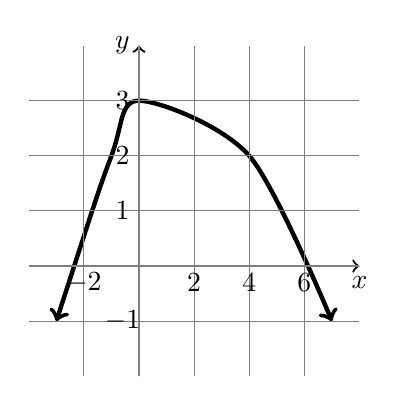
\begin{tikzpicture}[scale=.7]
\draw [ultra thick, <->] plot [smooth] coordinates {(-1.5,-1) (-.5,2) (0,3) (2,2) (3.5,-1)};
\draw[thick, ->] (-2,0) -- (4,0);\draw[thick, ->] (0,-2) -- (0,4);
\node at (4,-.3){$x$}; \node at (-.3,4){$y$};
\foreach \i in {-1,0,1,2,3}{
	\draw[gray] (-2,\i) -- (4,\i); \draw[gray] (\i,-2) -- (\i,4);
	}
\node at (-1,-.3){$-2$};\node at (1,-.3){$2$};\node at (2,-.3){$4$};\node at (3,-.3){$6$};
\node at (-.3,-1){$-1$};\node at (-.3,1){$1$};\node at (-.3,2){$2$};\node at (-.3,3){$3$};
\end{tikzpicture}

\item For the function $f(x)=\frac{2}{x}$, find the expression $f(12+h)-f(12).$ Simplify your answer and write your answer as a single fraction.\\

\item Given the piecewise defined function below, determine the value(s) of $x$ such that $f(x)=-20.$

$f(x)=\begin{cases} 2x+3 & x <0 \\ x^3 & x \geq 0 \end{cases}.$\\

\item Solve for $x$ in the equation $x^2+3x=10.$

\item Solve for $x$ in the equation $e^{4-7x}=\frac{1}{2}.$

\item Find all solutions to the equation $2\cos (\theta) = 1$ in the interval $[0, 2 \pi].$\\

\item A table of values for the function $f(x)$ is given below. Use the table to determine $f^{-1}(5).$

\begin{tabular}{|c||c|c|c|c|c|c|c|c|c|}
$x$&-5&0&5&10&15&20&25&30&35\\
\hline
$f(x)$&100&50&25&10&5&2&1&-1&-1/5\\
\end{tabular}

\item Solve the inequality $16-x^2\leq 0.$ Give your answer in interval notation.\\

\item Determine the domain of $f(x)=\ln(x-4).$ Give your answer in interval notation.\\

\item In the triangle below, $\sin \theta = \frac{2}{5}.$ Determine $\cos \theta.$ \\ 
 
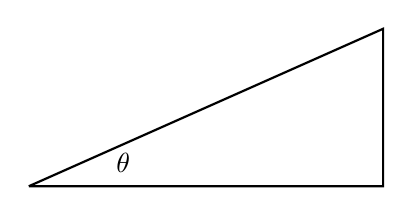
\begin{tikzpicture}
\draw[thick] (0,0)--(4.5,2) -- (4.5,0)-- (0,0);
\node at (1.2,.3){$\theta$};
\end{tikzpicture} \hfill \underline{\hspace{2in}}

\noindent Sketch graphs of the following functions. Label the $x$- and $y$-intercepts, if they exist. Draw in any asymptotes using dashed lines, and write the equation of the asymptote, if it exists.\\


\item $f(x) =(x+1)^3$

\item $f(x) = 1+e^{x} $ 

\item $y =\cos(x)$ on the interval $[-2\pi, 2\pi]$

%% WA 1.3 # 11
\item Given the graph of $f(x)$ below, draw the graph of $-2f(x).$

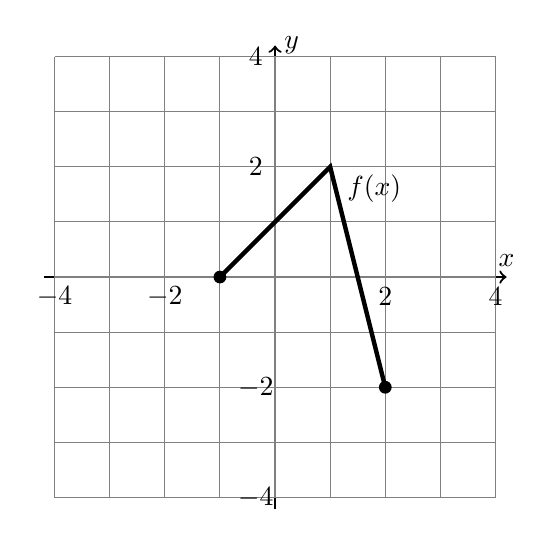
\begin{tikzpicture}[scale=.7]
\draw[thick, ->] (-4.2,0) -- (4.2,0);\draw[thick, ->] (0,-4.2) -- (0,4.2);
\node at (4.2,.3){$x$}; \node at (.3,4.2){$y$};
\foreach \i in {-4,-3,...,4}{
	\draw[gray] (-4,\i) -- (4,\i); \draw[gray] (\i,-4) -- (\i,4);

	}
\foreach \i in {-4,-2,2,4}{
	\node at (\i,-.35){$\i$};
	\node at (-.35,\i){$\i$};
	}
\node at (1.8, 1.6) {$f(x)$};
\draw[ultra thick] (-1,0) -- (1,2) -- (2,-2);	
\filldraw (-1,0) circle (3pt); \filldraw (2,-2) circle (3pt);
\end{tikzpicture}
%
\hspace{1cm}
%
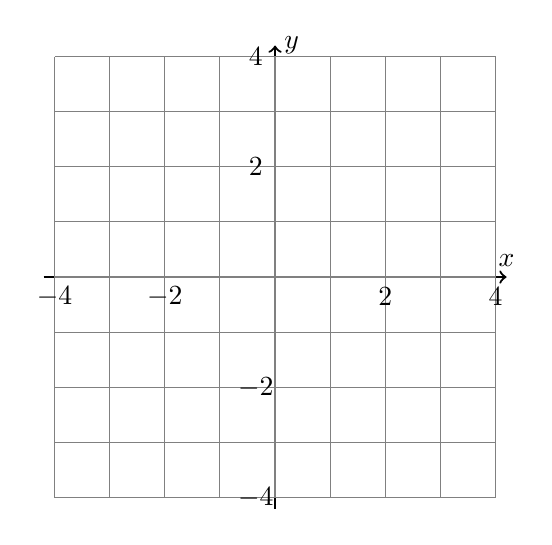
\begin{tikzpicture}[scale=.7]
\draw[thick, ->] (-4.2,0) -- (4.2,0);\draw[thick, ->] (0,-4.2) -- (0,4.2);
\node at (4.2,.3){$x$}; \node at (.3,4.2){$y$};
\foreach \i in {-4,-3,...,4}{
	\draw[gray] (-4,\i) -- (4,\i); \draw[gray] (\i,-4) -- (\i,4);

	}
\foreach \i in {-4,-2,2,4}{
	\node at (\i,-.35){$\i$};
	\node at (-.35,\i){$\i$};
	}
\end{tikzpicture}


\end{enumerate}
\end{document}
